% Based on docs/ambiguities/template.tex.
% Build from repository root: make questions LECTURE=13
\documentclass[a4paper,12pt]{article}
\usepackage[margin=19mm]{geometry}
\usepackage{amsmath,amssymb,graphicx,xcolor}
\usepackage{fontspec}
\usepackage{xepersian}
\settextfont{XB Roya}
\setlatintextfont{Latin Modern Roman}
\definecolor{ink}{HTML}{173D75}
\graphicspath{{images/}}
\setlength{\parindent}{0pt}
\setlength{\parskip}{4pt}
\linespread{1.08}
\newcommand{\qtitle}[2]{{\Large\bfseries\color{ink} پرسش \lr{#1}: #2}\par}
\newcommand{\answer}{\vfill\textbf{پاسخ یا صورت مورد تأیید و تاریخ:}\par\vspace{12mm}\hrule\medskip}
\begin{document}
{\LARGE\bfseries پرسش‌های ابهام جلسهٔ ۱۳}\par
{\large طول یک مدول؛ جزوهٔ جبر پیشرفتهٔ دکتر خسروی}\par
شمارهٔ صفحه‌ها، شمارهٔ یک‌مبنای صفحه در فایل پی‌دی‌اف است، نه شمارهٔ دست‌نویس.
\medskip\hrule\medskip

\qtitle{L13-Q01}{توان خودهمریختی در لم فیتینگ}
\textbf{وضعیت:} باز؛ برای بازبینی اختیاری بعدی. هنوز پاسخی ثبت نشده است.\par
\textbf{نشانی منبع:} نسخهٔ \lr{primary}، صفحهٔ ۸، صورت قضیه در بالای صفحه
و انتخاب توان در پایان اثبات همان صفحه.
\begin{LTR}\small\texttt{sources/lectures/13 Length of a Module.pdf}\end{LTR}
\textbf{صورت دست‌نویس:} اگر \(M\) یک \(R\)-مدول با طول \(n\) باشد و
\(f:M\to M\) یک \(R\)-همریختی، آنگاه
\[
 M=\operatorname{Im}f^n\oplus\ker f^n.
\]
\begin{center}
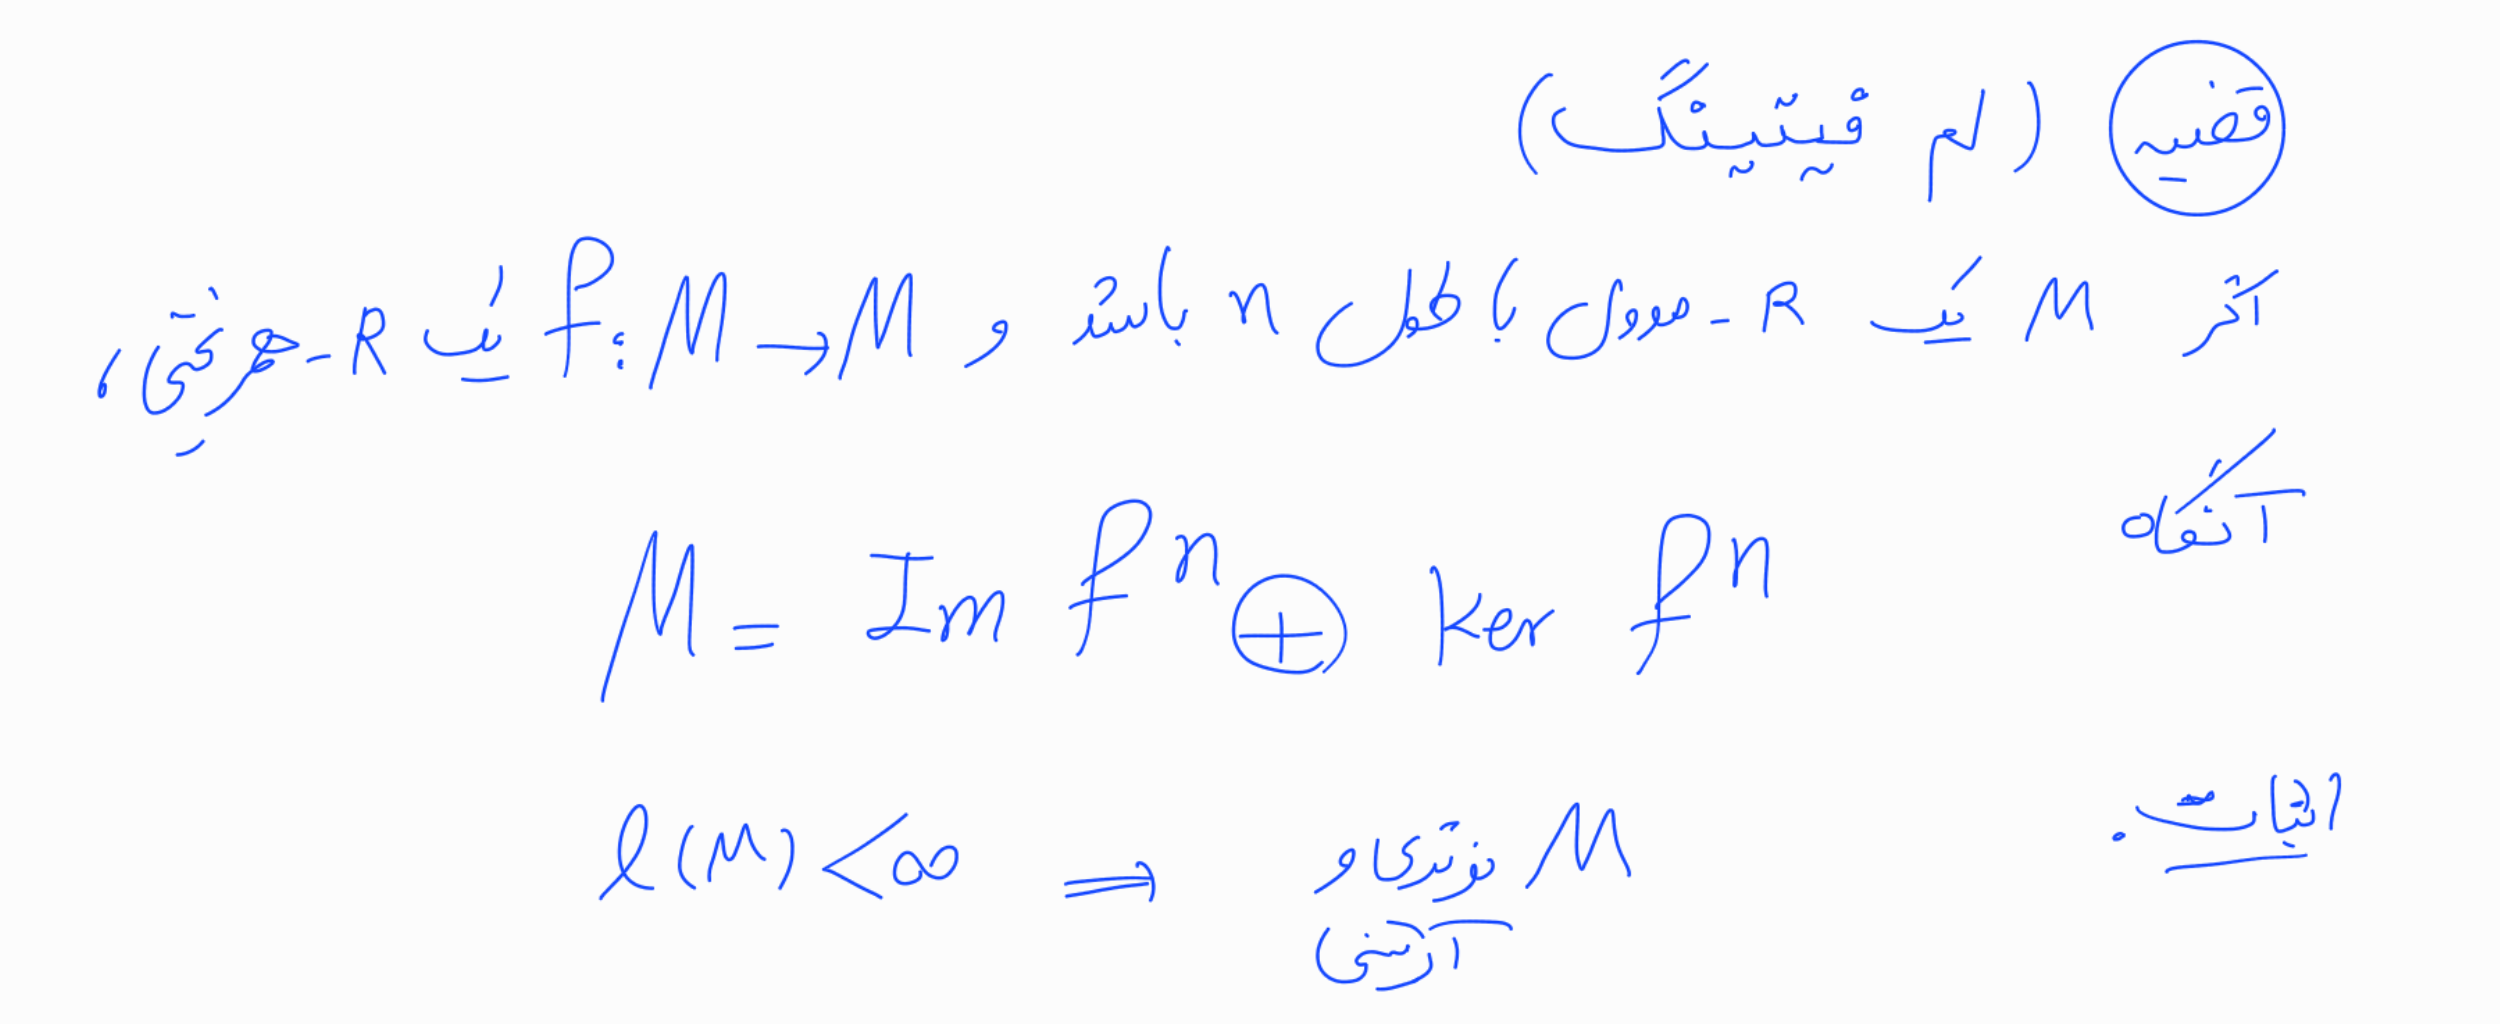
\includegraphics[width=\linewidth,height=35mm,keepaspectratio]{L13-Q01-statement.png}
\end{center}
\textbf{در اثبات:} ابتدا توان‌های توقف تصویر و هسته با \(n\) و \(k\)
مشخص شده‌اند. سپس برای \(m\geq\max\{n,k\}\)، توقف هم‌زمان نتیجه می‌شود.
\begin{center}
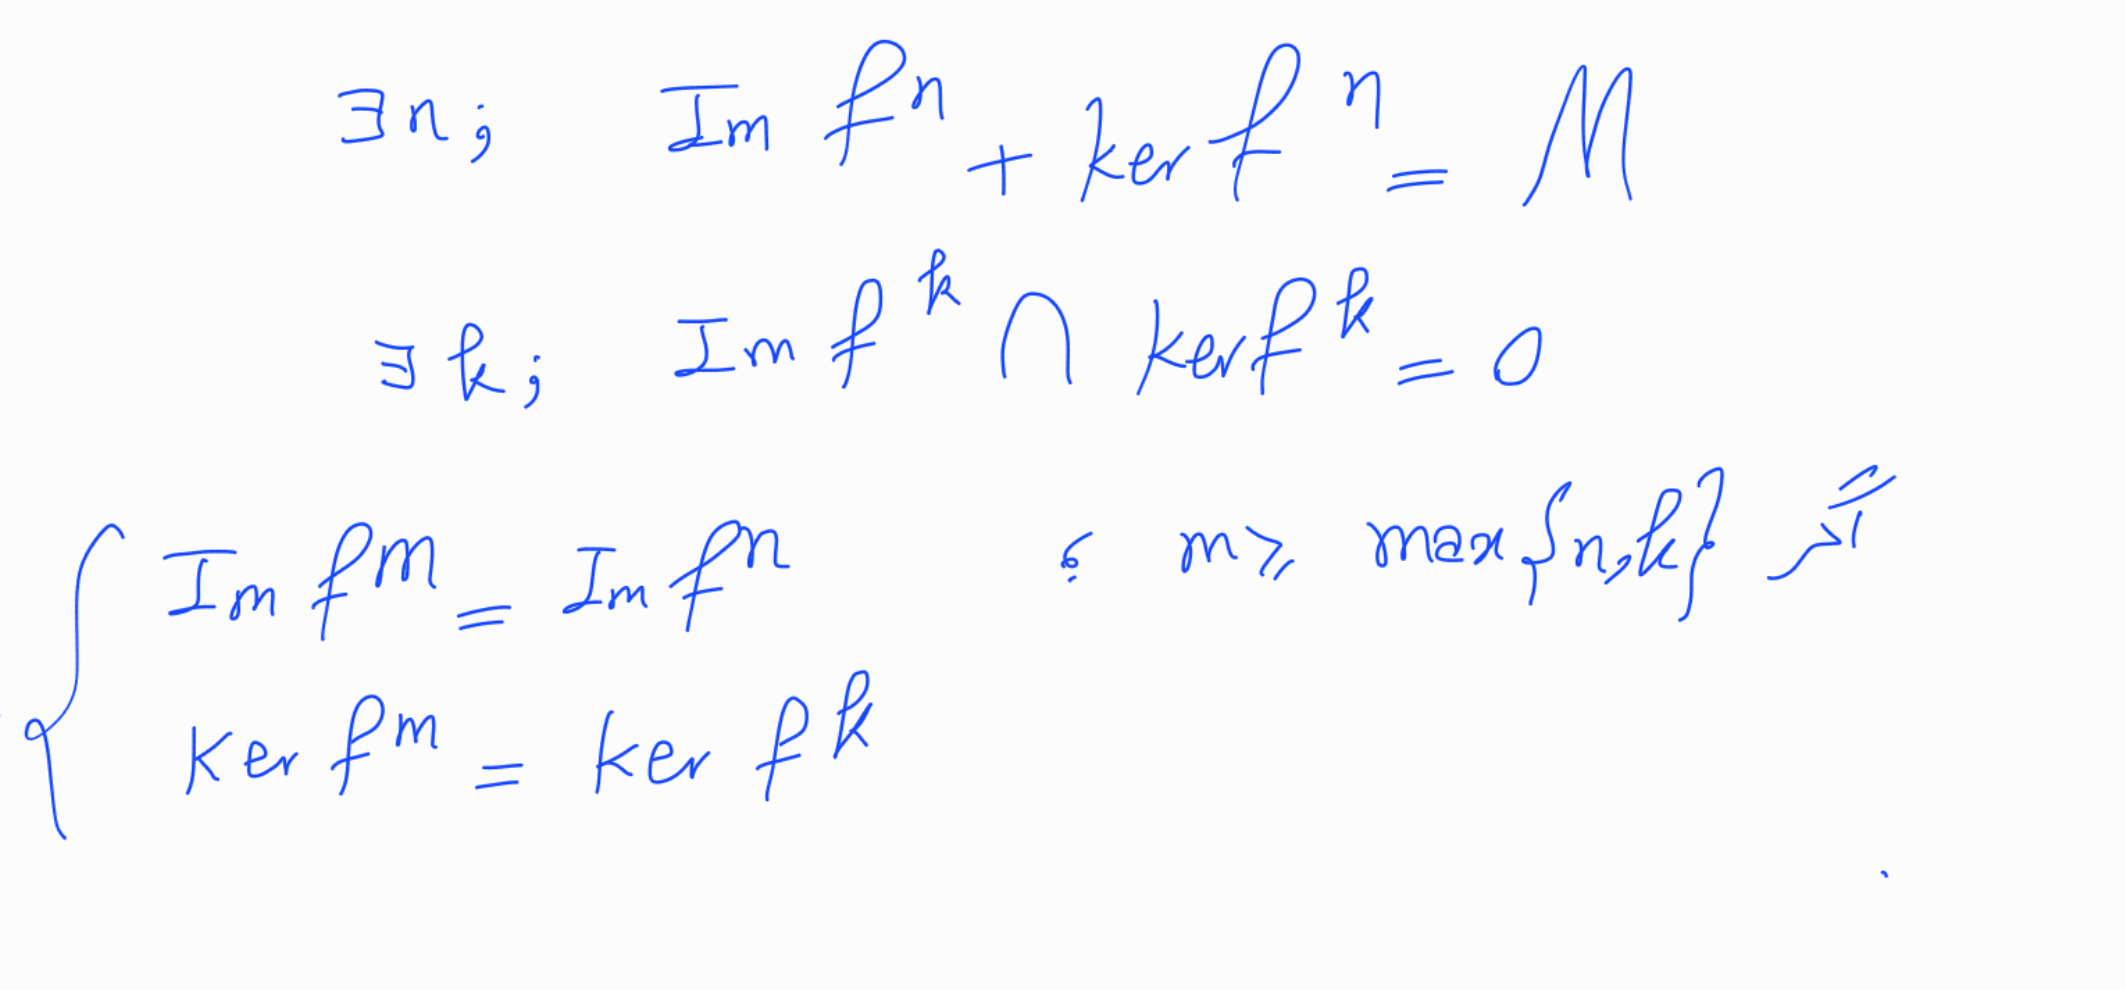
\includegraphics[width=.88\linewidth,height=37mm,keepaspectratio]{L13-Q01-proof.png}
\end{center}
\textbf{دو صورت قابل بررسی:} توانِ \(n=\ell(M)\) در خود صورت قضیه حفظ شود؛
یا صورت قضیه با یک توانِ به‌اندازهٔ کافی بزرگ نوشته شود.
اثبات ثبت‌شده، کران توان‌های توقف با \(\ell(M)\) را تصریح نمی‌کند.
این تفاوت، هم صورت قضیه و هم مقدار توضیح لازم در اثبات را تغییر می‌دهد.

\textbf{پرسش برای بازبینی بعدی:} آیا توان دقیقاً \(n=\ell(M)\) مقصود است،
یا «هر توانِ به‌اندازهٔ کافی بزرگ»؟ در حالت نخست، استدلالِ کرانِ توان‌های
توقف با \(\ell(M)\) در کدام گامِ جزوه منظور شده است؟

\textbf{روش این گذر:} صورت با توانِ برابر طول، موقت علامت خورده است؛
اثباتِ توانِ به‌اندازهٔ کافی بزرگ منتقل شده و استدلالِ کرانِ ذکرنشده
صریحاً به بازبینی بعدی واگذار شده است. گذر رونویسی با این پرسش باز پایان یافته است.
هر پاسخِ بعدی همراه تغییر و تاریخ ثبت خواهد شد.
\answer
\end{document}
